
\section{Statistical Methods}
\noindent{\em The first 3 rules of statistics: 'Draw a picture, Draw a picture, Draw a picture.'---Michael Starbird.}  


R~is a popular
programming/scripting language that is designed to make advanced
statistical analysis accessible.  Because of its ease of use, large user base, and
extensive community development, it is increasingly used by
researchers, statisticians, and data analysts from fields as varied as
economics, machine learning, pharmaceuticals, and finance.  The yearly
useR! conference boasts a sponsor list that includes such diverse
companies as Google, American Credit Acceptance, and the American
Statistical Association.  Virtually all of the most
influential and popular statistical and machine learning algorithms,
including Boosting, the LASSO, and random forests, have associated R
packages, often written by the inventors of the algorithms.  Although
it is difficult to obtain an exact number of R~users, a New York Times
article from 2009 estimated that there are at least 250,000 active R
users, with the number rising each year.  The RStudio company
develops a variety of software technologies, including an integrated
development environment (IDE) and server-side support for running R
programs remotely, that combine to make R~a painless and appealing
programming environment.  Finally, an increasing number of industrial actors, including
Oracle and Revolution Analytics, have begun offering support for R,
helping it gain industrial users.  R~therefore encompasses all the
necessary statistical models for morphometry, linear mixed effects
modeling and machine learning---supplemented with ANTs, we also gain
the necessary image processing core.


\begin{figure}{t}
\begin{center}
  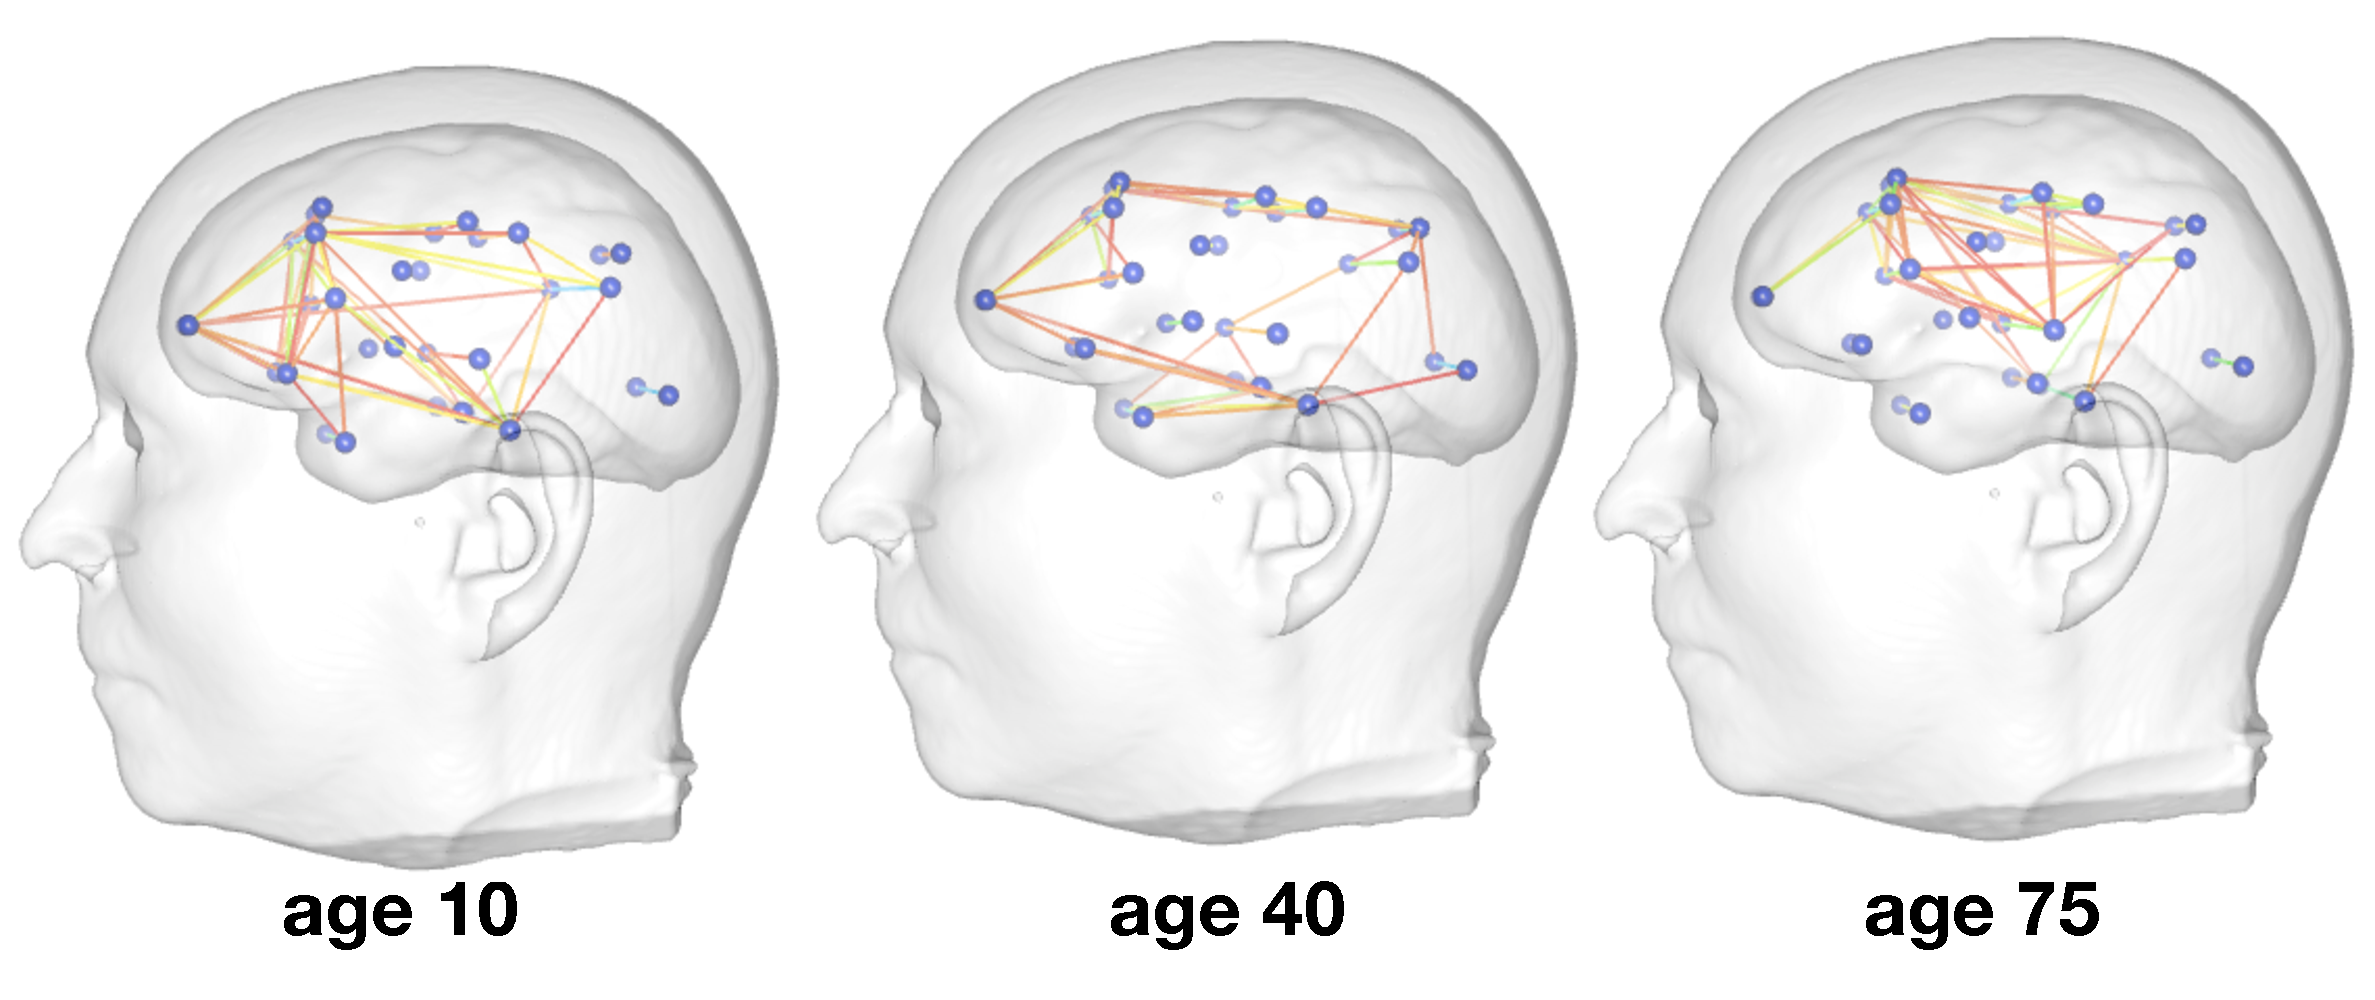
\includegraphics[width=0.45\textwidth]{figs/connx_age}
\end{center}
\caption{ANTsR connectivity analysis shows significant aging effects
  across structural brain networks (n=1200, from public IXI, OASIS, NKI datasets).}\label{fig:cnx}
\end{figure}

Ben --- need R writeup for basic morphometry / correlation-type studies i.e. use of
lm etc .... a model similar to: 
\begin{align}
\label{eq:eig2}
  \text{Outcome} \approx \text{Eig}([ \Delta \text{Volume} ]) [
  \beta_J ] + \\ \notag \text{Eig}([ \Delta \text{CBF} ]) [
  \beta_{\Delta  C} ] + \text{Eig}([ \Delta \text{FA} ]) [
  \beta_{\Delta  F} ] \notag + \\ \notag
~\text{Age}~\beta_d + ~\text{Sex}~\beta_g,
\end{align}
% \textcolor{red}{Why isn't 'education' not already folded into 'Predicted Pathology' as presumably 'age' and 'gender' have?}
where $\Delta$ represents a {\em linear} change measure and volumetric
change over time is measured by log-Jacobian \cite{Rohlfing2006}.  

Should we do this voxel-wise or using the Eig function?

